\section{Introduction}
\label{sec:intro}

Neural networks have undergone rapid development in various computer vision tasks such as image classification, detection and segmentation. While their impressive performance has powered many applications, a roaring trend is to pursue fast neural networks with low latency and high throughput for great user experiences, instant responses, safety reasons, etc.

How to be fast? Instead of asking for more costly computing devices, researchers and practitioners prefer to design cost-effective fast neural networks with reduced computational complexity, mainly measured in the number of {\bf fl}oating-point {\bf op}eration{\bf s} (FLOPs)\footnote{We follow a widely adopted definition of FLOPs, as the number of multiply-adds~\cite{zhang2018shufflenet,liu2022convnet}.}. MobileNets~\cite{howard2017mobilenets,sandler2018mobilenetv2,howard2019searching},
ShuffleNets~\cite{zhang2018shufflenet,ma2018shufflenet} and GhostNet~\cite{han2020ghostnet}, among others, leverage the depthwise convolution (DWConv)~\cite{sifre2014rigid} and/or group convolution (GConv)~\cite{krizhevsky2012imagenet} to extract spatial features. However, in the effort to reduce FLOPs, the operators often suffer from the side effect of increased memory access. MicroNet~\cite{li2021micronet} further decomposes and sparsifies the network to push its FLOPs to an extremely low level. Despite its improvement in FLOPs, this approach experiences inefficient fragmented computation. Besides, the above networks are often accompanied by additional data manipulations, such as concatenation, shuffling, and pooling, whose running time tends to be significant for tiny models.

\begin{figure}
    \centering
    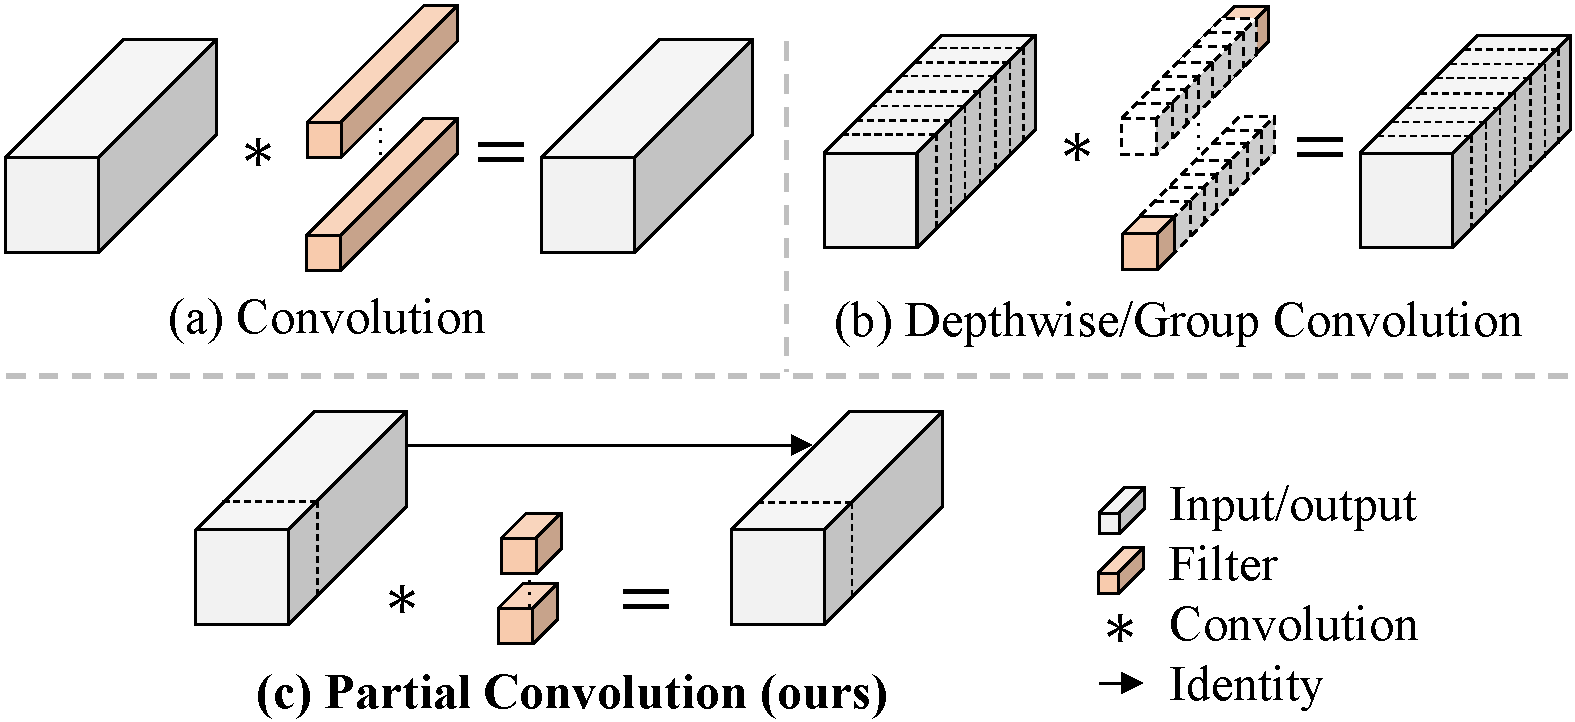
\includegraphics[width=1\linewidth]{figures/PConv-cropped.pdf}
    \vspace{-0.2in}
    \caption{Our partial convolution (PConv) is fast and efficient by applying filters on only a few input channels while leaving the remaining ones untouched. PConv obtains lower FLOPs than the regular convolution and higher FLOPS than the depthwise/group convolution.}
    \label{fig: PConv}
    \vspace{-0.05in}
\end{figure}

\begin{figure*}
    \centering
    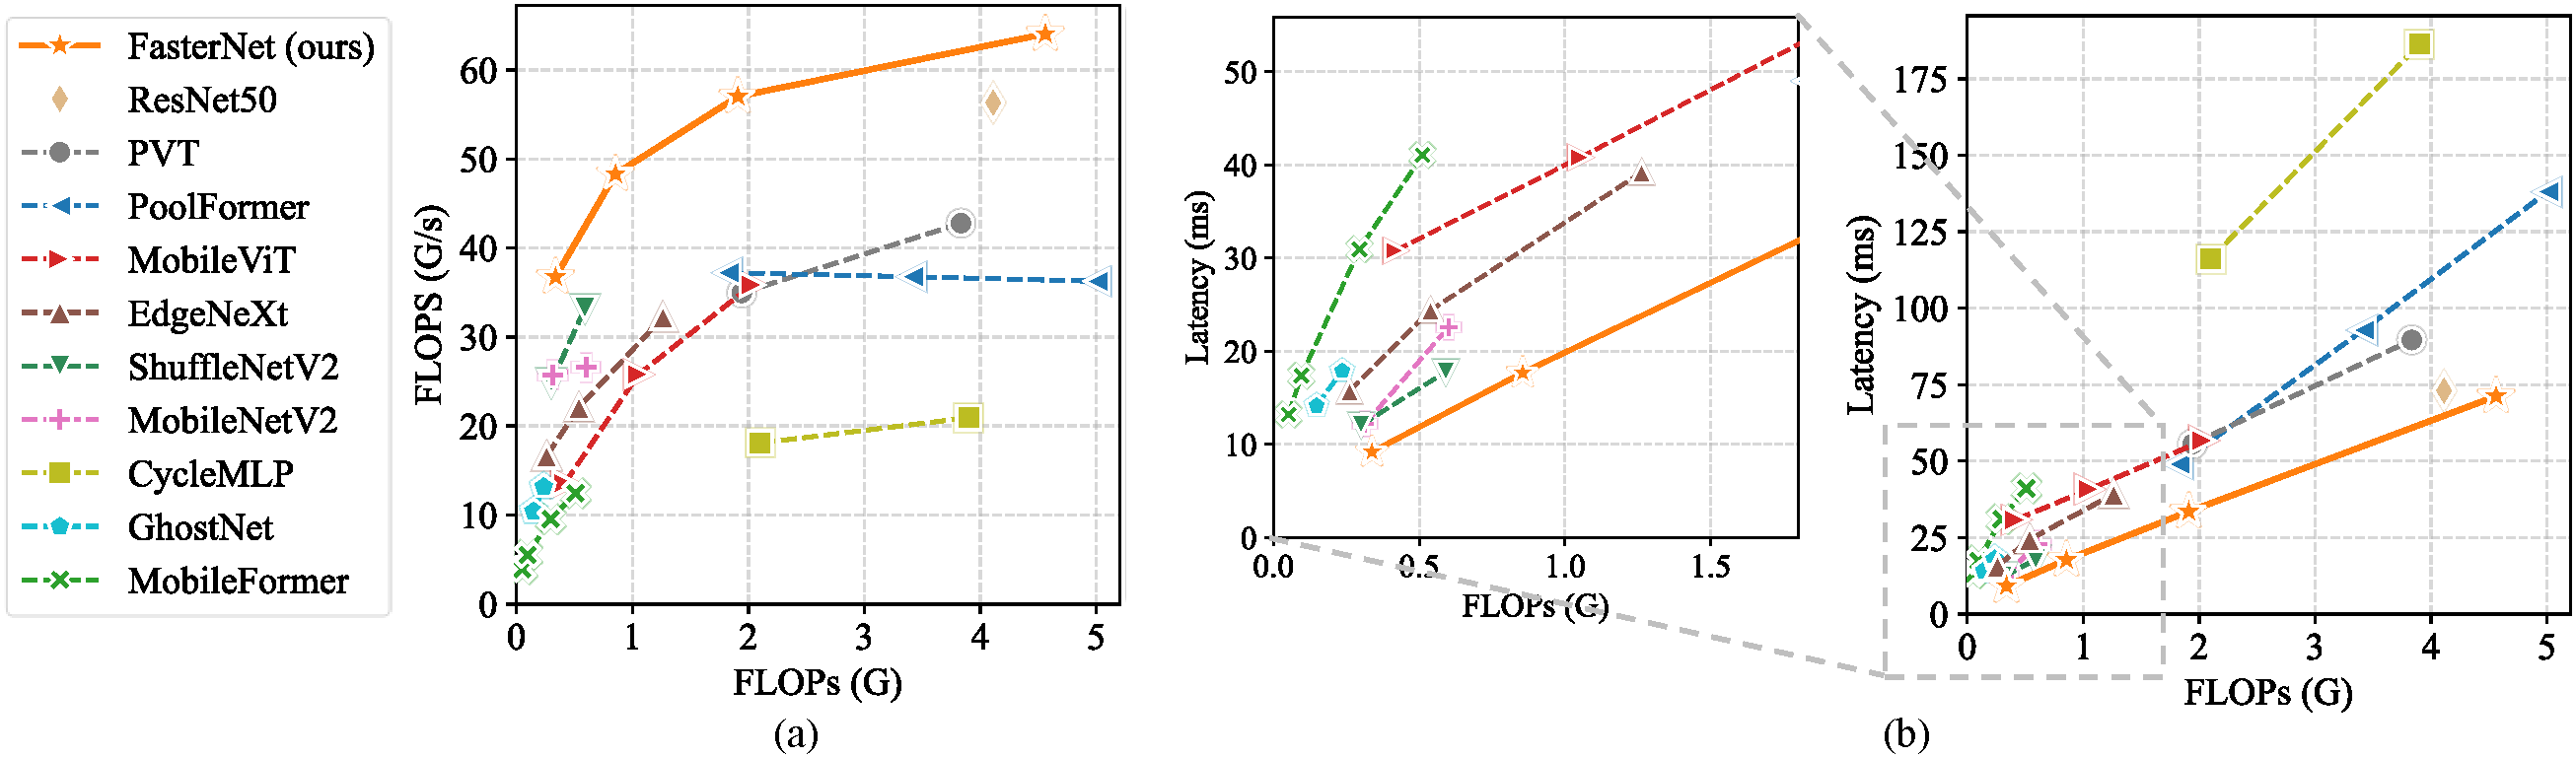
\includegraphics[width=1\linewidth]{figures/FLOPS_latency_vs_FLOPs-cropped.pdf}
    \vspace{-0.3in}
    \caption{(a) FLOPS under varied FLOPs on CPU. Many existing neural networks suffer from low computational speed issues. Their effective FLOPS are lower than the popular ResNet50. By contrast, our FasterNet attains higher FLOPS. (b) Latency under varied FLOPs on CPU. Our FasterNet obtains lower latency than others with the same amount of FLOPs.}
    \label{fig:FLOPS(latency)_vs_FLOPs}
    \vspace{-0.05in}
\end{figure*}

Apart from the above pure convolutional neural networks (CNNs),  there is an emerging interest in making vision transformers (ViTs)~\cite{dosovitskiy2020image} and multilayer perceptrons (MLPs) architectures~\cite{tolstikhin2021mlp} smaller and faster. For example, MobileViTs~\cite{mehta2021mobilevit,mehta2022separable,wadekar2022mobilevitv3} and MobileFormer~\cite{chen2022mobile} reduce the computational complexity by combining DWConv with a modified attention mechanism. However, they still suffer from the aforementioned issue with DWConv and also need dedicated hardware support for the modified attention mechanism. The use of advanced yet time-consuming normalization and activation layers may also limit their speed on devices.

All these issues together lead to the following question: Are
these ``fast'' neural networks really fast? To answer this, we examine the relationship between latency and FLOPs, which is captured by 
\begin{equation}
  Latency = \frac{FLOPs}{FLOPS},
  \label{eq:latency_FLOPs}
\end{equation}
where FLOPS is short for {\bf fl}oating-point {\bf op}erations per {\bf s}econd, as a measure of the effective computational speed. While there are many attempts to reduce FLOPs, they seldom consider optimizing FLOPS at the same time to achieve truly low latency. To better understand the situation, we compare the FLOPS of typical neural networks on an Intel CPU. The results in~\cref{fig:FLOPS(latency)_vs_FLOPs} show that many existing neural networks suffer from low FLOPS, and their FLOPS is generally lower than the popular ResNet50. With such low FLOPS, these ``fast'' neural networks are actually not fast enough.
Their reduction in FLOPs cannot be translated into the exact amount of reduction in latency. In some cases, there is no improvement, and it even leads to worse latency. For example, CycleMLP-B1~\cite{chen2021cyclemlp} has half of FLOPs of ResNet50~\cite{he2016deep} but runs more slowly (\ie, CycleMLP-B1 \vs ResNet50: 116.1ms \vs 73.0ms). Note that this discrepancy between FLOPs and latency has also been noticed in previous works~\cite{ma2018shufflenet,mehta2021mobilevit} but remains unresolved partially because they employ the DWConv/GConv and various data manipulations with low FLOPS. It is deemed there are no better alternatives available.

This paper aims to eliminate the discrepancy by developing a simple yet fast and effective operator that maintains high FLOPS with reduced FLOPs. Specifically, we reexamine existing operators, particularly  DWConv, in terms of the computational speed -- FLOPS. We uncover that the main reason causing the low FLOPS issue is \emph{frequent memory access}. We then propose a novel partial convolution (PConv) as a competitive alternative that reduces the computational redundancy as well as the number of memory access. \cref{fig: PConv} illustrates the design of our PConv. It takes advantage of redundancy within the feature maps and systematically applies a regular convolution (Conv) on only a part of the input channels while leaving the remaining ones untouched. By nature, PConv has lower FLOPs than the regular Conv while having higher FLOPS than the DWConv/GConv. In other words, PConv better exploits the on-device computational capacity. PConv is also effective in extracting spatial features as empirically validated later in the paper. 


We further introduce FasterNet, which is primarily built upon our PConv, as a new family of networks that run highly fast on various devices. In particular, our FasterNet achieves state-of-the-art performance for classification, detection, and segmentation tasks while having much lower latency and higher throughput. For example, our tiny FasterNet-T0 is $2.8\times$, $3.3\times$, and $2.4\times$ faster than MobileViT-XXS~\cite{mehta2021mobilevit} on GPU, CPU, and ARM processors, respectively, while being 2.9\% more accurate on ImageNet-1k. Our large FasterNet-L achieves 83.5\% top-1 accuracy, on par with the emerging Swin-B~\cite{liu2021swin}, while offering 36\% higher throughput on GPU and saving 37\% compute time on CPU. To summarize, our contributions are as follows:
\begin{itemize}
\itemsep0em 
\item We point out the importance of achieving higher FLOPS beyond simply reducing FLOPs for faster neural networks.
\item We introduce a simple yet fast and effective operator called PConv, which has a high potential to replace the existing go-to choice, DWConv.
\item We introduce FasterNet which runs favorably and universally fast on a variety of devices such as GPU, CPU, and ARM processors.
\item We conduct extensive experiments on various tasks and validate the high speed and effectiveness of our PConv and FasterNet.
\end{itemize}